\section{ITSA-58-1 計算正整數被3整除之數值之總和}
\centerline{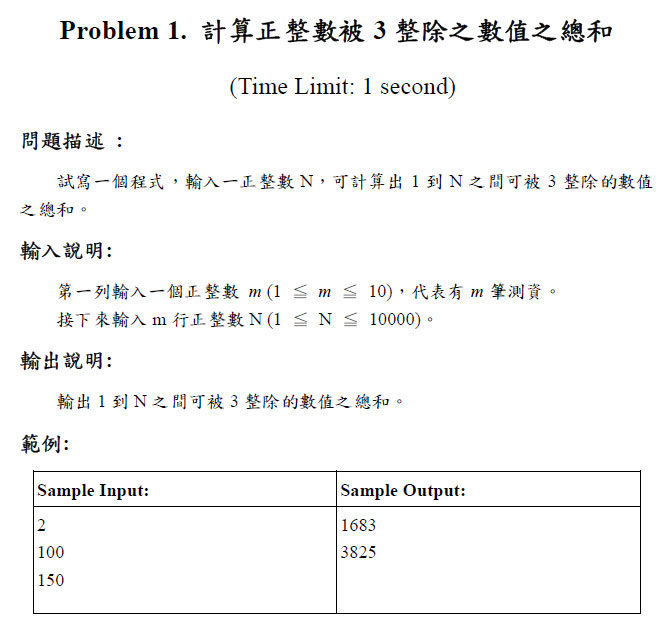
\includegraphics[width=.8\textwidth]{../solutions/fig/58ITSA1}}
\subsection{解題思惟}
\begin{enumerate}
	\item 如果有n個case要處理的話,可以設一個變數,例如kase,讀入n之後,用以下迴圈求解,剛好會跑n次。
	\begin{inside}
		int kase; cin >> kase;
		while (kase--) {
			// 處理一個case
		}
	\end{inside}
	\item 求和的話,可以設一個變數,例如sum=0,然後把要加的都加到sum裡面。
	\item 從1檢查到n的話,可以跑一個for迴圈,像下面這樣:
	\begin{inside}
		for (int i=1; i<=n; i++) {
			// 處理i的情況
		}
	\end{inside}
	\item 檢查i是否為3的倍數,就把i除以3看餘數是否為0,是0的話,i就是3的倍數。
	\begin{inside}
		if (i%3==0) sum += i; // i是3的倍數
	\end{inside}
\end{enumerate}
\subsection{程式碼}
\begin{cppcode}
#include <iostream>

using namespace std;

int main()
{
	int kase, n; cin >> kase;
	while (kase--) {
		cin >> n;
		int sum = 0;
		for (int i=1; i<=n; i++) {
			if (i%3==0) sum += i;
		}
		cout << sum << endl;
	}
	return 0;
}
\end{cppcode}
